\subsubsection{Iteration 2: Supporting Learning through UI and Tutorial}

\paragraph{Design}

The findings from the previous iteration indicated that participants were initially unable to understand the controller-based interaction. Therefore, this iteration focused on improving learnability through structured tutorials, enhanced visual feedback, and environmental constraints.

The system was extended with three primary interaction components: (1) the Quad GameObject, representing the physical quadcopter model; (2) the DroneVision GameObject, which uses Unity's RenderTexture to provide a first-person view (FPV) through a virtual headset; and (3) the Instruct GameObject, which delivers step-by-step tutorial guidance. The structure of the scene is illustrated in \cref{fig:tutorial_scene}.

\begin{figure}[H]
    \caption{Components of the Tutorial Scene}\label{fig:tutorial_scene}
    \centering
    \begin{tikzpicture}
        % 建议先定义类，再用 umlpackage 包含，或确保坐标明确
        \begin{umlpackage}{Tutorial Scene}
            \umlclass[width=3cm]{Quad}{
                + FpvCam: Camera
            }{
            }
            
            \umlclass[x=6, width=4cm]{DroneVision}{
                - renderTexture : RenderTexture
            }{}
            
            \umlclass[y=-3, x=3, width=4cm]{Instruct}{
                - tutorialSteps : List
            }{
                + Next()
            }
            
            % 连线需放在 package 内部或紧随其后
            \umluniassoc{DroneVision}{Quad}
            \umluniassoc{Instruct}{Quad}
            \umluniassoc{Instruct}{DroneVision}
        \end{umlpackage}
    \end{tikzpicture}
\end{figure}

The Quad GameObject functions as the physical simulation of the quadcopter, while DroneVision renders the onboard camera feed to simulate FPV piloting. The Instruct module presents content in a sequential manner, covering arming, throttle, yaw, pitch, and roll control. During tutorial execution, the quadcopter's Rigidbody is temporarily locked to support reflective observation, consistent with Kolb's experiential learning cycle \parencite{kolb1984}.

To improve interaction awareness, a dual-layer HUD system was introduced. A cross-axis indicator was rendered in front of the player, while corresponding visual markers were placed within the scene to represent real-time joystick input positions.

In total, six interaction modes were implemented. Five correspond to quadcopter flight control in mode 2 \cref{fig:mode2}, while one supports general XR interaction:

\begin{itemize}
    \item \textbf{Arm}: Activates the rotor system by pulling the left joystick to its minimum position.
    \item \textbf{Throttle}: Controls vertical thrust by adjusting the vertical axis of the left joystick.
    \item \textbf{Yaw}: Controls rotational movement around the vertical axis via horizontal movement of the left joystick.
    \item \textbf{Pitch}: Controls forward and backward tilt using the vertical axis of the right joystick.
    \item \textbf{Roll}: Controls lateral tilt using the horizontal axis of the right joystick.
    \item \textbf{Grip/Select}: Enables interaction with UI elements using the controller grip button.
\end{itemize}

Additionally, the DroneXrEmulator \cref{fig:quad_structure} was extended with a BoxCollider parameter to define a bounded safe flight area.

\paragraph{Enactment}

The updated system maintained a video-passthrough XR environment while introducing structured abstractions that map directly to real-world drone control inputs. The tutorial system guided users through incremental interaction learning, while the HUD provided continuous feedback of controller input states. The inclusion of a bounded flight space ensured that users remained within a safe operational area during early learning stages.

\begin{figure}[H]
    \caption{Structure of the interaction system components}\label{fig:interact}
    \centering
    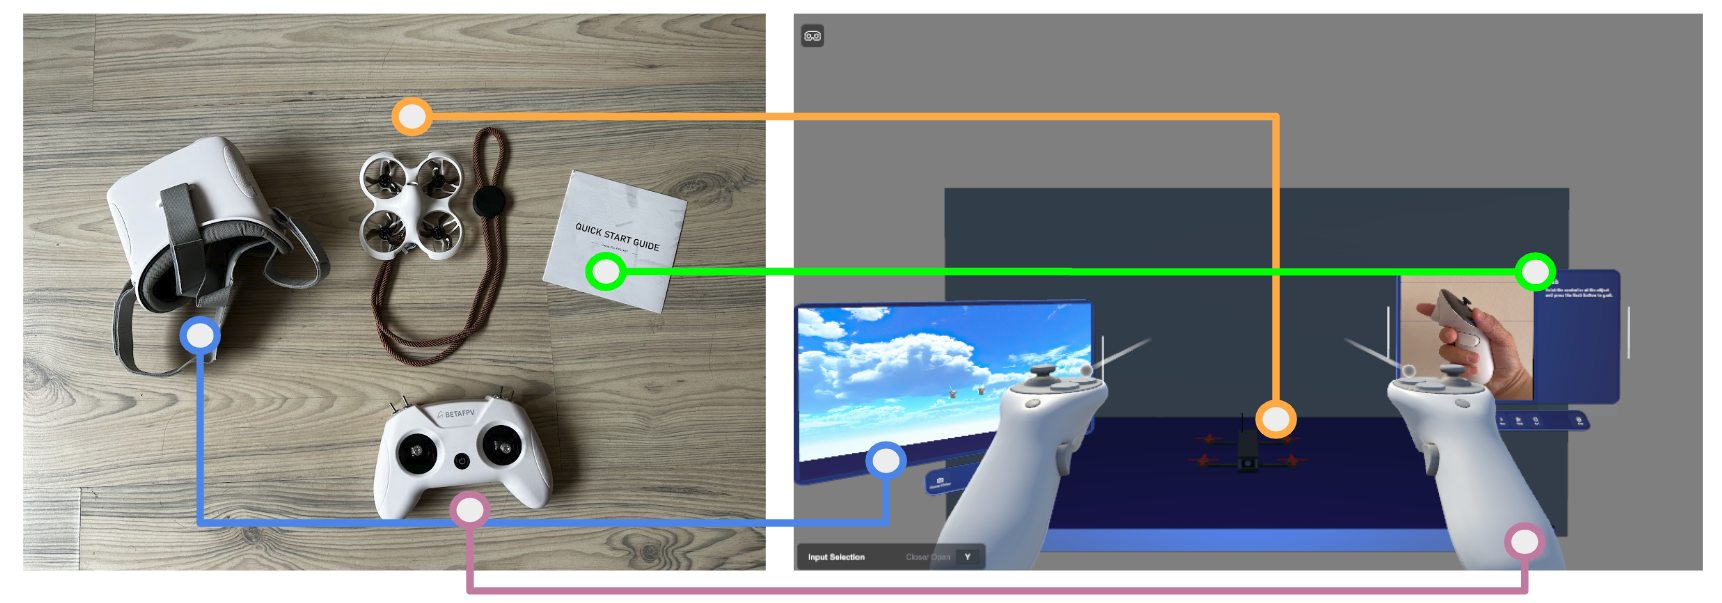
\includegraphics[width=0.8\linewidth]{img/stages/structure.png}
\end{figure}

\paragraph{Analysis}

Observational testing showed that participants were able to understand basic controller interactions in third-person mode after the introduction of the tutorial system. However, difficulties persisted in spatial orientation during FPV (DroneVision) mode. In particular, the skydome environment did not provide sufficient directional cues, which negatively impacted navigation performance in first-person piloting scenarios.